\chapter{METHODOLOGY: METRICS AND DIAGNOSTIC FIELDS}
\label{ch:methods}


%The analysis will focus on three main characteristics of cyclones commonly utilized \cite{deshpande2010impact, bopape2021sensitivity,  zarzycki2021metrics, nyongesa2024influence, mishra2024characteristics} in weather forecasting: track, intensity, and rainfall. The table below outlines the questions designed to guide the examination of each characteristic in alignment with the dissertation's objectives. This approach will help refine the metrics and outputs available in the existing literature.

Our methodology is designed based on three main characteristics of tropical cyclones commonly utilized in weather forecasting: track, intensity, and rainfall. The metrics that are currently used in similar studies will be described accordingly to each category. Then, for each hurricane, a table with addressed questions will be shown to guide the reader in the analysis and discussion of the results. This table will be part of the workflow, a diagram that shows the steps and figures/maps that will be created. 
All code made for this dissertation is available on the
\href{https://github.com/biancafusi/Dissertation}{GitHub - Dissertation Repository}, mainly written in Python.

\begin{center}
\captionof{table}{Key Research Questions for Track, Intensity, and Rainfall Assessment } \label{tab:questions}
 % Título centralizado acima
\end{center}

\begin{longtable}{p{2.5cm} p{10cm} p{1.5cm}}
\textbf{Topic} & \textbf{Question} & \textbf{ID} \\
\hline
\endfirsthead

\textbf{Topic} & \textbf{Question} & \textbf{ID} \\
\hline
\endhead

\multicolumn{3}{r}{\textit{Table continued on next page}} \\
\endfoot

\hline
\endlastfoot

Trajectory & What is the overall performance of the parameterization and sensitivity tests in reproducing the hurricane's track? & T.1 \\
& What is the error (in kilometers) associated with these tracks? & T.2 \\
& Which configuration shows the best performance? & T.3 \\
& After how many forecast hours do larger deviations begin to appear? & T.4 \\
& Is there any observable trend in the tracks? & T.5 \\
& How does the large-scale environment influence these deviations? & T.6 \\
& What is the overall performance of MONAN? & T.7 \\
\hline
Intensity & What is the overall performance of the parameterization and sensitivity tests in reproducing the hurricane's intensity? & I.1 \\
& How much bias is present in these results? & I.2 \\
& How well does ERA5 perform in reproducing this intensity, and why? & I.3 \\
& Is there any thermodynamic or mechanical explanation for these trends? & I.4 \\
& What is the overall performance of MONAN? & I.5 \\
\hline
Rainfall & What is the overall performance of the parameterization and sensitivity tests in reproducing the hurricane’s rainfall pattern? & R.1 \\
& In which regions is there a negative (or positive) bias in the rainfall field? & R.2 \\
& What is the overall performance of the parameterization and sensitivity tests in reproducing the hurricane’s cloud morphology? & R.3 \\
& How much light, moderate, and heavy rainfall is being produced by the simulations? & R.4 \\
& What is the average rainfall produced by the simulations? & R.5 \\
& What is the bias between the extreme rainfall produced by the simulations and the reference data? & R.6 \\
& What is the overall performance of MONAN? & R.7 \\
\end{longtable}

\begin{center}
Source: Made by the author (2025).
\end{center}

%In the following subsections, the approaches and metrics used to evaluate each of these characteristics will be explained in detail. Finally, a workflow diagram will be presented, summarizing the described methods and indicating at which stage each question will be addressed.
%All code made for this dissertation is available on the git repository: \href{https://github.com/biancafusi/Dissertation}{GitHub - Dissertation Repository} mainly written in Python

\section{Trajectory}

A map illustrating the forecasted trajectories will be generated using a tracking algorithm developed by the author. A discussion regarding the performance of this tracking and guidance can be found in Appendix \ref{appendixB}. Additionally, a time series analysis will be conducted to evaluate the errors associated with each trajectory. These errors are defined as the distance between the central pressure reference points and the forecasted central pressure points, calculated using the GeoPy library\footnote{\href{https://geopy.readthedocs.io/en/stable/}{https://geopy.readthedocs.io/en/stable/}}. As noted in the literature, the calculations could be performed following the methodology proposed by \citeonline{moon2021five} but here we simply calculate the great-circle distance between two points. 

To quantitatively validate the results, a graphical representation will display the Mean Absolute Error (MAE) and Root Mean Square Error (RMSE) for each of the trajectories, regarding the reference dataset.

The MAE is widely employed \cite{ditchek2023improving, nyongesa2024influence} in the literature and can be defined as:

\begin{equation}
    \text{MAE} = \frac{1}{N}\sum_{i=1}^{N} |F_i -O_i|
\end{equation}

\noindent in this equation, $N$ represents the sample size (number of points in the trajectory), $F$ denotes the forecast outputs generated by the model, and $O$ refers to the observation outputs obtained from a reference dataset. The error values can range from 0 to $\infty$, with a perfect score indicated by 0. The aim is to calculate the average magnitude of the forecast errors. It is important to note that this error does not convey the direction of the deviations due to its absolute nature; this aspect will be examined using another method discussed later.

Along with the MAE, usually, RMSE is computed to seek a kind of average error, but now weighted according to the square of the error. As the same as before, it varies from 0 to $\infty$, and a perfect score means RMSE equal to 0. It is defined as:

\begin{equation}
    \text{RMSE} = \sqrt{\frac{1}{N}\sum_{i=1}^{N} (F_i -O_i)^2}
\end{equation}

The letters in this equation have the same meaning as in the previous equation. To better understand the potential trends in the trajectory, in addition to visual comparisons, one can utilize cross-track and along-track errors computed into a time series. The errors assess the deviation of the forecasted position from the observed path (cross-track) and the speed of the forecast from the observations (along-track). The cross-track error is measured perpendicularly to the observed trajectory, while the along-track error is measured along the actual course at a specified event. Together, these metrics\footnote{The equations used to compute those errors can be found at this website: \url{https://www.movable-type.co.uk/scripts/latlong.html}} can also indicate the directional error of each forecast. Figure~\ref{fig:cross-along-errors} more clearly illustrates the distinction between cross-track and along-track errors. 

\begin{figure}[htbp]
    \centering
    \caption{Illustration of cross-track and along-track errors. The definitions of Cross-Track Error (CTE) and Along-Track Error (ATE) are based on the distance between an observation (obs) and a forecast (fct) at the same valid time (T). This distance is computed as the great-circle distance.} % Título acima
    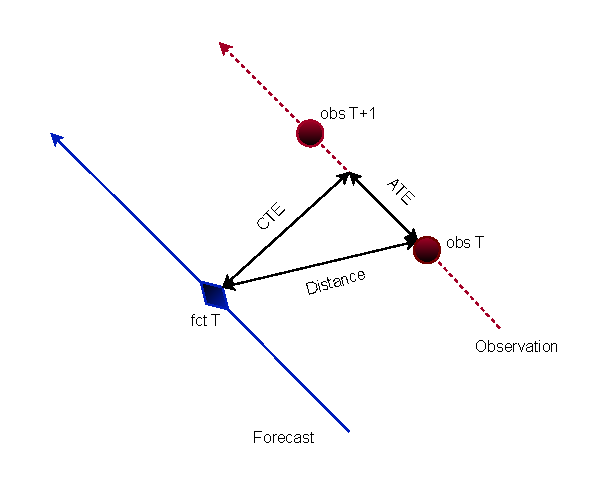
\includegraphics[width=0.8\textwidth]{docs/figuras/chapter4/cte_ate.pdf} 
    \label{fig:cross-along-errors}
    \vspace{0.5em}
    
    \centering
    Source: Made by the author (2025).
\end{figure}

In the context of our expected findings, negative (positive) values of cross-track errors indicate that the forecasted center of the hurricane is projected to be located to the west (east), while negative (positive) values of along-track errors suggest that the center is slower (faster) than its intended trajectory.

Those errors can be clarified by examining the meteorological fields. Following the approach of \citeonline{gao2023regulating}, analyzing the 700 hPa geopotential height can reveal the large-scale features contributing to the bias in the trackings. For instance, in the authors' study, forecasts displaying significant eastward track bias for tropical cyclones often correspond with a noticeably weaker subtropical high over the North Atlantic. These fields can be computed easily using Python.

In conclusion, utilizing a straightforward statistical mean of the errors (specifically the MAE and RMSE) can provide valuable insights into the overall performance of the MONAN simulations. The mean is defined as follows:

\begin{equation}
    \text{MEAN} = \frac{1}{E} \sum_{i=1}^{E} errors_i
\end{equation}

where E denotes the total number of experiments conducted using the MONAN framework. This approach facilitates a comprehensive understanding of the general behavior exhibited by the MONAN runs and can be compared with ERA5, for instance.

%%%%%%%%%%%%%%%%%%%%%%%%%%%%%%%%%%%%%%%%
\section{Intensity}

In reviewing the literature, tropical cyclone intensity is defined as the maximum surface wind speed associated with the central pressure \cite{demaria2007evaluation, landsea2013atlantic}. However, some studies argue that depending exclusively on wind speed does not fully capture the concept of intensity, suggesting that pressure can also serve as a significant indicator of forecasted intensity \cite{shepherd2017sensitivity, heming2017tropical}. This dissertation will adopt the latter approach by evaluating both pressure and wind as intensity indicators.

To conduct these evaluations, we will analyze time series data that includes the central pressure identified by the tracking system and the maximum wind speed, which is derived from the first level of the model. A discussion on how to determine this maximum wind speed in the model can be found in Appendix~\ref{appendixA}. The time series will serve as a measure of forecast performance, allowing us to assess how closely the computed values align with actual observations and where they occur.

In addition to a visual comparison, we will create a graph containing the MAE and RMSE to quantify the forecasts and rank them based on their effectiveness in illustrating intensity. Additionally, the mean of those errors can also be computed and compared with ERA5 to give us insights into the general MONAN performance. 

To validate these results, we can examine meteorological fields such as the geopotential height between 850 hPa and 500 hPa, as well as the pressure and wind fields at 850 hPa, to gain insights into the forecast's impact on cyclone movement and intensity; all of the fields can easily be computed using Python. 

%%%%%%%%%%%%%%%%%%%%%%%%%%%%%%%%%%%%%%%%%%%
\section{Rainfall}

The analysis of rainfall for our runs is based on the methodology proposed by \citeonline{marchok2007validation}. According to these authors, evaluating forecasted rainfall requires examining three key aspects: the rainfall pattern, the mean and distribution of rain volume, and the extreme values.


To investigate the rainfall pattern, we will utilize the Equitable Threat Score (ETS; \citeonline{mesinger2008bias}) along with pattern correlation analysis (namely the Pearson Correlation Coefficient) and visual comparisons using selected snapshots, considering also the related bias of those fields. The mean and distribution of rain volume can be assessed through the computation of the Cumulative Density Function (CDF) and the Probability Density Function (PDF). Extreme rainfall values will be specifically analyzed by examining the 85th percentile computed at the CDF. Lastly, we will discuss a performance score for MONAN in comparison to ERA5 by averaging the results of all experiments. Table~\ref{tab:rainfall_metrics} summarizes the metrics to be computed, followed by a brief explanation of each metric and its intended purpose.

\begin{table}[H]
\centering
\caption{Metrics used to evaluate rainfall forecast performance}
\label{tab:rainfall_metrics}
\resizebox{\textwidth}{!}{
\begin{tabular}{lp{11cm}}
\toprule
\textbf{Metric} & \textbf{Definition} \\
\midrule
ETS (Equitable Threat Score) & Measures the skill of categorical forecasts by comparing the number of hits to what would be expected by chance:
\[
\text{ETS} = \frac{H - H_r}{H + F + M - H_r}
\]
where \(H\) is the number of hits, \(F\) is false alarms, \(M\) is misses, and \(H_r = \frac{(H+F)(H+M)}{total}\) is the expected number of hits due to chance. \\

Pearson Correlation Coefficient & Measures the spatial similarity between observed and forecasted rainfall fields:
\[
r = \frac{\sum_{i=1}^{n} (F_i - \bar{F})(O_i - \bar{O})}{\sqrt{\sum_{i=1}^{n} (F_i - \bar{F})^2 \sum_{i=1}^{n} (O_i - \bar{O})^2}}
\]
where \(F\) and \(O\) are forecasted and observed values, calculated over $n$ data points, where $i$ is the index running from 1 to $n$. \\

Bias & Quantifies the difference between forecast and observation:
\[
\text{Bias} = F - O
\] \\

CDF (Cumulative Distribution Function) & Represents the probability that a variable takes a value less than or equal to a given threshold:
\[
\text{CDF}(x) = P(X \leq x)
\] \\

PDF (Probability Density Function) & Describes the relative likelihood for a variable to take a specific value:
\[
\text{PDF}(x) = \frac{d}{dx} \, \text{CDF}(x)
\] \\
\bottomrule
\end{tabular}
}
\vspace{0.3cm}
\centering
Source: Made by the author (2025).
\end{table}

The ETS evaluates how well forecasted “yes” events correspond to observed “yes” events, while accounting for agreements due to random chance. According to \citeonline{marchok2007validation}, this implies that the ETS penalizes a model for overproducing rainfall above a given threshold, even if the rainfall pattern is realistic. For this metric, a hit is defined as an event that was forecasted to occur and did occur; a miss is an event that was not forecasted but occurred; and a false alarm is an event that was forecasted but did not occur.

Pattern correlation is computed as the Pearson correlation coefficient (r) between the forecasted and observed rainfall fields. The correlation ranges from -1 to 1, where: ($i$) $r = 1$ indicates a perfect positive linear relationship; ($ii$) $r = -1$, a perfect negative linear relationship; and ($iii$) $r = 0$ implies no linear relationship between forecast and observation.

The bias is the difference between the forecast ($F$) and the observations ($O$), typically averaged over time or space. A negative bias indicates underestimation, while a positive bias indicates overestimation. The bias can range from negative to positive infinity, with 0 representing a perfect forecast.

Both the CDF and the PDF will be used to analyze rainfall distributions. The CDF shows the cumulative probability of rainfall values up to a certain threshold. For example, the corresponding x-axis value when the y-axis equals to 0.5 (or 50\%) on the CDF corresponds to the median rainfall amount. The CDF ranges from 0 to 1 on the y-axis, indicating the proportion of the data below a given threshold on the x-axis. For instance, the 0.85 mark on the CDF corresponds to the 85th percentile, meaning 85\% of the data falls below that threshold, and the remaining 15\% above it. This is a straightforward way to seek for rainfall extremes.

The PDF, similar to a histogram, describes the probability of observing values within a specific range. It is normalized such that the total area under the curve equals 1. To interpret the PDF, one can compute the area under the curve within a specified range, which represents the probability of a value falling in that interval. Mathematically, the CDF is the integral of the PDF. One should notice that both CDF and PDF can be computed empirically or theoretically. The difference between them is that when computing empirically, one will consider the natural distribution of data, and theoretically, one will consider a mathematical distribution (gamma, Gaussian, etc). In this study, we will utilize the empirical approach.



%%%%%%%%%%%%%%%%%%%%%%%%%%%%%%%%%%%%%%%%%%%%%
\section{Hurricane Beryl workflow}

The workflow below summarizes and organizes the upcoming steps. After a quick initial analysis, the results will be visually represented as trapezoidal shapes, while discussions will be depicted with rectangular shapes. This distinction helps clarify the types of information being presented at each stage of the process. Following this, the boxes containing question IDs, as outlined in Table~\ref{tab:questions}, related to the three aspects under evaluation (trajectory, intensity, and rainfall) will be also displayed in the workflow.

\begin{figure}[p]
    \centering
    \caption{Workflow Overview}
    \label{fig:workflow}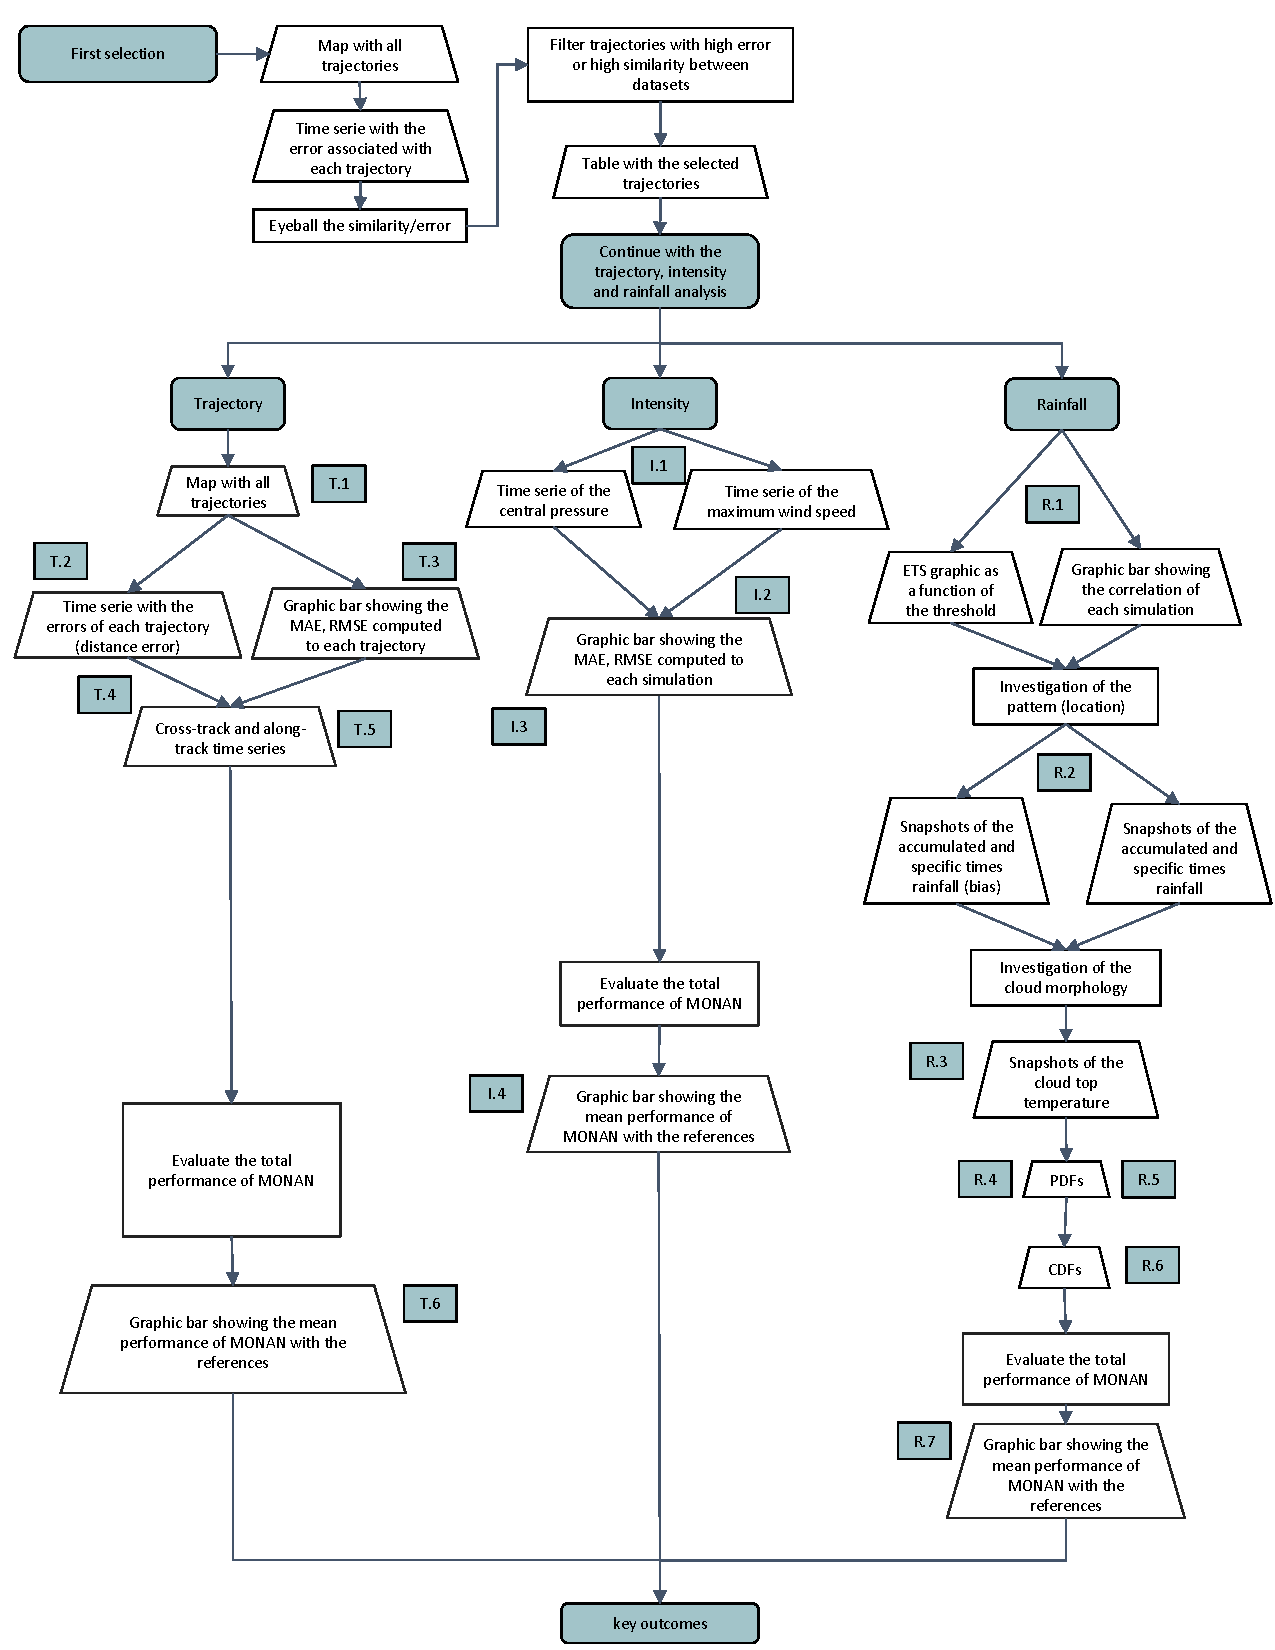
\includegraphics[width=\textwidth,height=\textheight,keepaspectratio]{docs/figuras/chapter4/BERYL_worflow_01.pdf}

    \vspace{0.5em}
    
    \centering
    Source: Made by the author (2025).
\end{figure}

The reader should note that an initial selection of the results will be conducted. As the diagram indicates, a trajectory map will be created, accompanied by distance errors. The selection criteria will focus on experiments that do not contribute significantly to the discussion, either because they are part of a set of similar experiments or due to excessively large errors that do not accurately represent the model state we aim to address.

\section{Hurricane Helene workflow}